
\documentclass[a4paper,12pt]{article}
\usepackage[utf8]{inputenc}
\usepackage{graphicx}
\usepackage[magyar]{babel}
\usepackage{t1enc}

\begin{document}

\author{Elek István}

\title{Giwer \linebreak \linebreak GeoImage Workflow Editing Resources  \linebreak  \linebreak \small Felhasználói leírás \linebreak \linebreak}


\date{2022 július}


\setcounter{tocdepth}{3}
%\frontmatter
\maketitle
\newpage
\tableofcontents
\newpage
%\mainmatter


\section*{Bevezetés}

A \textbf{Giwer} rendszer (GeoImage Workflow Editing Resources) egy képfeldolgozó rendszer, amely űrfelvételek és légi fotók feldolgozására alkalmas. Ez a felhasználói leírás megismertet a rendszer használatával. Először bemutatjuk a főbb funkciókat. Ebben a leírásban a keretrendszert, a \textbf{DataStock}, a \textbf{Catalog} és a \textbf{WorkflowBuilder} alrendszert mutatjuk be. 

Az ED\_18-1-2019-0030 szerződésszámú projekt (Alkalmazásiterület-specifikus nagy megbízhatóságú informatikai megoldások)  a Nemzeti Kutatási Fejlesztési és Innovációs Alapból biztosított támogatással, a Tématerületi kiválósági program finanszírozásában valósult meg.



\section{A Giwer rövid bemutatása}

\subsection{A keretrendszer}

Egy keretprogram vezérli a különböző programrészeket, modulokat. Ez a \textbf{giwer.exe} nevű program. Célja a a rendszer működésének irányítása. Segítségével indíthatjuk el a különböző modulokat, a \textbf{catalog.exe}-t, \textbf{dataStock.exe}-t, és a \textbf{workflowBuilder.exe}-t (szerkesztőt és futtatót). 

Itt indíthatjuk el a programok konfigurálását végző programrészt (Config), valamint a program használatát segítő leírást (Help), végül pedig a program metaadatait bemutató információs részt (Info).
A A \textbf{Catalog}, a \textbf{DataStock} és a \textbf{Workflow builder} önállóan is elindítható a keretrendszer nélkül, ha éppen úgy akarja a felhasználó.

\subsection{Catalog}

A képek igen nagy mennyiségben keletkeznek, így ezek áttekintése egy idő után lehetetlenné válik. Ezért létrehoztunk egy kép katalógust, egy nyilvántartó, kezelő alrendszert, amely adatbázisban tárolja, rendszerezi a képeket, ezáltal biztosítva az eligazodást, keresés a nagy mennyiségű kép között.

\subsection{Data stock}

Ez az alkalmazás egy interaktív működő képfeldolgozó rendszer. Számos függvényt implementáltunk, amelyek az adatok olvasását, írását, manipulálását végzik. Ezek a program menürendszerében jelennek meg, amit a felhasználó interaktívan, az egyes eljárások eredményességét vizsgálandó, aktivizálhat.


\subsection{Workflow builder}

Ezzel a modullal a rendelkezésre álló függvényekből tetszőleges munkafolyamatot (workflowt) állíthatunk elő, amelyet tárolhatunk, futtathatunk, szerkeszthetünk. A workflow csak az összeállított eljárásokat tartalmazza, így futtatáskor meg kell adnunk, hogy mely adatcsoportokra kívánjuk futtatni. Ezek lehetnek egy-egy képfájl, vagy sok képből álló projekt.


\subsection{Config}

A \textbf{Config} editorral, amelyet a keretprogramból indíthatunk el, a rendszer adatforrásait állíthatjuk be (\ref{fig:config}. ábra). Megadhatjuk, hogy hol találhatjuk a fájlrendszerben az idegen formátumú adatokat (\textit{bil}, \textit{tif}, \textit{jpg}, \textit{3D}), és a rendszer saját adatformátumú fájljait (\textit{gwh}), a projekteket(\textit{prj}) és a workflowkat (\textit{wkf}). 
 
 \begin{figure}[h]
 	\centering
 	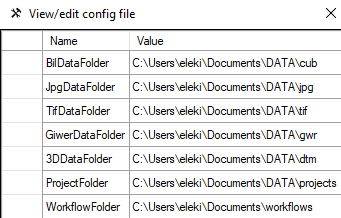
\includegraphics[width=6cm]{config.png}
 	\caption{A \textbf{Config} viewer/editor}
 	\label{fig:config}
 \end{figure}
 

A kiválasztott nevű paraméter (\textit{Name}) nem változtatható meg, csak az értéke (\textit{Value} mező), ha ráklikkelünk a megfelelő sor \textit{Value} mezőjére. A változások mentése a \textit{config.cfg} nevű text fájlba történik az \textit{Enter} lenyomásával vagy a következő sorra lépéssel. \textit{Config.cfg} a \textbf{giwer.exe} fájlt tartalmazó könyvtárban van. Ezt a fájlt nem tanácsos kézzel editálgatni, kivéve, ha valaki pontosan tudja, hogy mit csinál, mert könnyen hibát idézhet elő a program futása során.



\subsection{Help}

A rendszer használatát users' guide-ok támogatják, amelyek a \textit{Help} ikonnal aktivizálhatók. Itt kiválaszthatjuk, hogy melyik alrendszert szeretnénk megismerni, mivel külön users' guide áll rendelkezésre a \textbf{Giwer/DataStock}, a \textbf{Catalog} és \textbf{Workflow builder} alrendszerekhez. Ugyaninnen indíthatunk tutorialokat is.


\subsection{Info}

Az \textit{Info} ikonra klikkeléssel a rendszer metaadatait nézhetjük meg (szerzők, évszámok, verziószámok, copyright, néhány mondatos leírás, jogok stb.)
%\\
%\newpage


\section{A keretrendszer}

\begin{figure}[h]
	\centering
	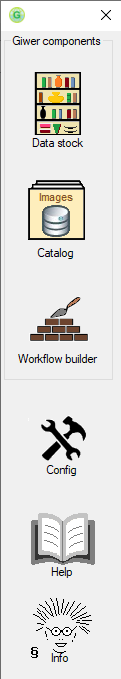
\includegraphics[height=13.5cm]{giwerMain.png}
	\caption{A \textbf{Giwer} keretrendszer}
	\label{fig:giwerStart}
\end{figure}

A keretrendszer arra szolgál a \textbf{Giwer} programrendszer különböző komponenseit összefogja. Noha az alrendszerek önállóan is futtathatók, de a keretrendszer révén jobban áttekinthetővé válik a működés. A \textit{Giwer.exe} elindítása után megjelenik \textit{Giwer components} című ablak (\ref{fig:giwerStart}. ábra), ahol hat nagyméretű ikon látható. Az első a \textit{DataStock}-ot, a második a \textit{Catalog}-ot indítja, a harmadik a  \textit{WorkflowBuilder}-t, a többi a keretrendszer része. A \textit{Config} ikonnal a rendszer paramétereit állíthatjuk, vagyis hol találhatók a különböző az adataink (\ref{fig:config}. ábra). A \textit{Help} egy külön ablakban megjeleníti a felhasználói kézikönyveket és a tutorialokat alrendszerenként, az \textit{Info} ikon pedig egy bemutatkozó ablakot jelenít meg a programról.




\section{DataStock}

A \textbf{Giwer} rendszer interaktív modulja a \textbf{DataStock}, ami a menürendszeren keresztül teszi elérhetővé a függvénykönyvtárat és az adatokat. Különböző típusú grafikus fájlok (\textit{bil, tif, jpg}) beolvasását és manipulálását végzi. Speciális, saját fájlformátuma a \textit{GWR/GWH} formátum. A \textit{GWH} egy header fájl, amely az adott kép metaadatait tartalmazza, míg a \textit{GWR} egy bináris formátum, amely egységesen kezelhetővé teszi a legkülönbözőbb forrásokból származó adatokat, és lényegesen gyorsabbá teszi a feldolgozási műveleteket.

\subsection{Menürendszer}

A menürendszer (\ref{fig:datastock_fomenu}. ábra) \textit{File}, \textit{One band processes}, \textit{Multiband processes}, \textit{Data tools} és \textit{Workflow} menüelemekből áll, valamint  az aktuális \textit{Lookup table} beállítást mutatja (default, hypsometric, ndvi, user stb), amelyet szükség szerint átállíthatunk egy másikra. A \textit{default} beállítás greyscale megjelenítést végez. A \textit{hypsometric} egy 8 bites, maximum 256 színű színezést tesz lehetővé attól függően, hogy a \textit{lookup table}-ben hány színt állítottunk be. Ez a hagyományos hipszometrikus megjelenítés stílusa, amely az alacsony területeket a zöld árnyalataival, a kissé magasabb területek a sárga árnyalataival, és a magas területeket a barna árnyalataival jeleníti meg. Az \textit{ndvi} az ndvi számításkor használatos színes megjelenítést teszi lehetővé. A \textit{user} a felhasználó által beállított \textit{lookup table}-t mutatja, amelynek az osztályozáskor lesz jelentősége.

\begin{figure}
	\centering
	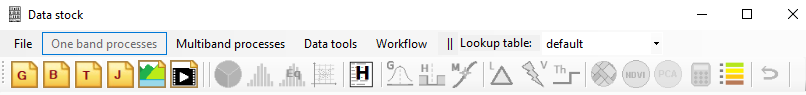
\includegraphics[width=14cm]{datastock_fomenu.png}
	\caption{A \textbf{datastock} fő menüje}
	\label{fig:datastock_fomenu}
\end{figure}

\subsubsection{File}

A \textit{File} menüvel (\ref{fig:filemenu_datastock}. ábra) meg tudunk nyitni \textit{gwh, bil, tif, jpg, ddm} típusú fájlokat, valamint projekt fájlokat, amelyek egyszerre több kép kezelésére szolgálnak. Törölhetjük valamely (akár több) \textit{gwh} fájlt. A \textit{gwh, gwr} fájlok a \textbf{Giwer} rendszer saját formátumú fájljai. Elmenthetjük egy feldolgozás eredményét giwer formátumban, vagy egyszerű bitmapként. 

Elmenthetjük továbbá projektként is a \textbf{Giwer}-ben lévő adatoknak azt az állapotát, ami egy adott pillanatban éppen fennáll. Ez olyankor célszerű, amikor sok képet szeretnénk egy időben nézegetni, manipulálni. A projekt fájl beolvasásával egyszerre olvashatjuk és tölthetjük be a réteglistára a képeket (\ref{fig:projectfile}. ábra). Ha egy réteglistát el akarunk menteni, mint projectet, akkor kattintsunk a \textit{Save project file} almenüre. A projekt fájl kiterjesztése \textit{prj}. A projekt jelentősége majd a \textbf{WorkflowBuilder} használatakor válik igazán fontossá. A projekt fájl egy egyszerű szövegfájl. Nem tanácsos editálgatni, mert olvashatatlanná válhat. Nem a végfelhasználónak készül, hanem a rendszernek.

\begin{figure}[h]
	\centering
	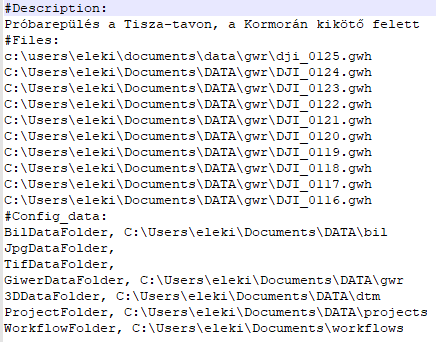
\includegraphics[width=7cm]{project_file}
	\caption{Példa egy projekt fájlra menü}
	\label{fig:projectfile}
\end{figure}

Végül pedig ismételten betölthetjük a rendszer konfigurációs adatait, ha időközben megváltoztattuk azt a keretprogrammal (nem frissül automatikusan).

\begin{figure}
	\centering
	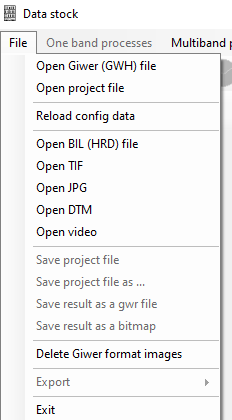
\includegraphics[width=4cm]{filemenu_datastock.png}
	\caption{A \textbf{File} menü}
	\label{fig:filemenu_datastock}
\end{figure}

 A képek beolvasása még nem jelent megjelenítést. Ehhez ki kell választanunk a megjeleníteni kívánt frekvenciasávot a \textit{Data stock} ablak \textit{Layers} fülén lévő valamelyik listaelemre kattintással (\ref{fig:layer_list}. ábra). A kiválasztás után a legtöbb menüelem és gyors gombok (főmenü alatti ikonok) aktív állapotba kerülnek.
 
\begin{figure}
	\centering
	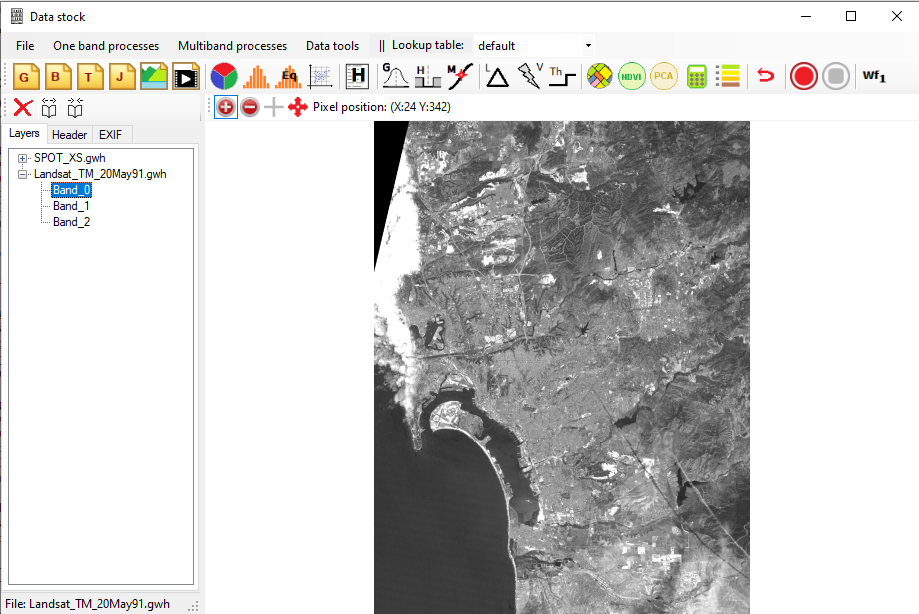
\includegraphics[width=14cm]{layer_list.png}
	\caption{Képek megjelenítése a \textit{Layer list} valamely elemének kiválasztásával}
	\label{fig:layer_list}
\end{figure} 
	
A \textit{gwh} egy text fájl, amely header tipusú adatokat tartalmaz a képről (szélesség, magasság, frekvenciasávok száma, bitmélység, stb.), míg a \textit{gwr} egy bináris fájl, amely pixeladatokat tartalmaz sorfolytonosan. 

A \textit{bil} fájl egy régi űrfelvétel formátum, amely szintén header fájlból és egy bináris fájlból áll. A *.hdr fájl a kép metaadatait, *.bil pedig a pixel adatokat tartalmaz. Részletes leírása megtalálható a \newline \textit{http://desktop.arcgis.com/en/arcmap/10.3/manage-data/raster-and-images/ bil-bip-and-bsq-raster-files.htm} weboldalon. 

A \textit{tiff, jpg} fájlok jól ismert képformátumok, amelyek különböző színmélységű és sávszámú képek tárolására alkalmasak.

A menüsor alatti ikonosztázon (gyors gombok) láthatók a leggyakoribb fájltípusok megnyitására szolgáló ikonok, mint például \includegraphics[width=0.5cm]{opengiwer.png} (open giwer file format, ami a gwh fájlt jelent), \includegraphics[width=0.5cm]{openbil.png} (open bil format), \includegraphics[width=0.5cm]{opentif.png} (open tif format), \includegraphics[width=0.5cm]{openjpg.png} (open jpg format), 
\includegraphics[width=0.5cm]{3d.png} (open 3D, egyelőre csak a magyar ddm formátmot érti) és \includegraphics[width=0.5cm]{openvideo.png} (open video).

	
\subsubsection{One band processes}

 
Ez a menü akkor használható, amikor egy kiválasztott frekvenciasávval kívánunk műveleteket végrehajtani. Kiválasztás után meg is jelenik a képablakban. %(\ref{fig:ug_datastock2}. ábra).
 A \textit{One band processes} menü elemei a következők: \textit{Histogram, Thresholding, Vectorizing, Filters, Texture, Segmentation, Clustering, Raster calculator} (\ref{fig:onebandmenu}. ábra).

\begin{figure}
	\centering
	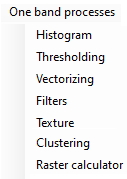
\includegraphics[width=3cm]{onebandmenu.png}
	\caption{A \textbf{One band processes} menü}
	\label{fig:onebandmenu}
\end{figure}

\begin{itemize}
	
	\item A \textit{Draw histrogram} almenü kirajzolja a kép hisztogramját, amelyet a kép kiegyenlítésére (kontrasztosítására) használhatunk. A bal egérgomb klikkel a minimális, a jobb egérgomb klikkel a maximális értéket választhatjuk ki. Az \textit{Equalize} gombbal elvégezzük a kiegyenlítést. 
%	Választhatjuk a \textit{Histrogram equalization} gombbal, hogy automatikusan választjuk ki a minimális és maximális értéket, és hajthatjuk végre a kiegyenlítést. Ilyenkor a hisztogram nem rajzolódik ki, csak az eredmény a képen.	
%	
	\item Ha a \textit{Histrogram equalization} menüre kattintunk, akkor automatikus választjuk ki a minimális és maximális értéket, és hajthatjuk végre a kiegyenlítést. Ilyenkor a hisztogram nem rajzolódik ki, csak az eredmény a képen.
	
	\item A \textit{Thresholding} küszöbölést hajt végre egy megadható küszöbértéktől függően. Általában más eljárásokkal kombinálva használható.
	
	\item A \textit{Vectorizing} vektoros jellegű adatot állít elő a képből. A nyers képre nem érdemes alkalmazni, mert az eredmény rossz lesz. Mielőtt alkalmaznánk, előtte simítószűrést, küszöbölést és éldetektálás (Laplace filter) kell végezni. 
		
	\item A \textit{Filters} egy több almenüből álló gyűjtemény, amely különböző szűrési eljárásokat (\textit{Gauss smoothing, High pass filter, Gradient filters, Laplace filter, Median filter}) végez a képen. 
		
	\item A \textit{Texture} menü az aktuális kép textúráját elemzi (fejlesztés alatt)
	
%	\item A \textit{Segmentation} menü az aktuális frekvenciasáv szegmentálását végzi.
	
	\item A \textit{Clustering} menü az aktuális frekvenciasáv  osztályozását végzi.
	
	\item A \textit{Raster calculator} menü leválogatja az aktuális frekvenciasáv azon pixeljeit, amelyek a megadott  feltételeket eleget tesznek.
	

\end{itemize}
	
	 
\subsubsection{Multiband processes}

A\textit{ Multiband processes} csoportba azok a funkciók tartoznak, amelyek egyszerre több frekvenciasáv adatait igénylik mint pl. RGB képek létrehozása, PCA (főkomponens analízis a megadott frekvenciasávokra), NDVI (vegetációs index), több frekvenciasáv alapján történő osztályozás, képek kombinálása, stb ( \ref{fig:multiband_menu}. ábra). 


	\begin{figure}
	\centering
	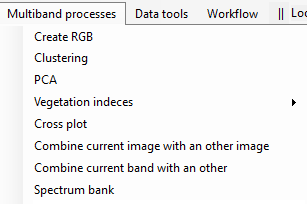
\includegraphics[width=7cm]{multiband_menu.png}
	\caption{A \textit{Multiband processes} menü}
	\label{fig:multiband_menu}
	\end{figure}


\begin{itemize}
	
	\item A \textit{Create RGB} menü RGB képet kreál a megadott három frekvenciasávból
	
	%\item A \textit{Segmentation} menü a kiválasztott frekvenciasávokra szegmentálást végez.
	
	\item A \textit{Clustering} menü a kiválasztott frekvenciasávokra osztályozást végez.
	
	\item A \textit{PCA} menü a kiválasztott frekvenciasávokra főkomponens analízist végez
	
	\item Az \textit{Vegetation indeces} menü a kiválasztott frekvenciasávokból vegetációs indexet számol.
	
	\item A \textit{Cross plot} menü a kiválasztott két frekvenciasávból cross plottot rajzol, és ez alapján grafikus szelektálást végez.
	
	\item A \textit{Combine current image with an other image} az aktuális képet kombinálja (+,-, EXOR) egy tetszőleges másik képpel. Ez olyankor hasznos, ha például egy vektorizált képet össze akarunk rajzolni az eredeti képpel (ekkor az EXOR operátort kell használni).
	
	\item A \textit{Combine current band with an other} Egyazon kép több frekvenciasávjának kombinálásra való
	
	\item A \textit{Spectrum bank} menü az elmentett spektrumbank szerkesztésére, elemzésére szolgál.
	

\end{itemize}

\subsubsection{Data tools}

A \textit{Data tools} menü az adatok előkészítésére való funkciókat tartalmazza (\ref{fig:datatools_menu}. ábra). Különböző formátumok konverzióját, egyesítését, kombinálást végzi. Néhány, a drón képek konverziójával kapcsolatos problémát old meg. A \textit{Lookup table} szerkesztését is lehetővé teszi. Legfontosabb funkciója azonban a \textit{Convert to Giwer format} almenü. Ennek segítségével bármely nyers képformátumot (bil, tif, jpg) giwer formátumba konvertálja. Tömeges konverzióra a \textit{Convert selected files to Giwer format} menü szolgál.

A giwer formátum kétféle fájlt jelent: a \textit{.gwr} egy vagy több bináris fájl, ami a képet tartalmazza frekvenciasávonként. Annyi fájl tartalmaz, ahány sávos a kép, (pl. 0.gwr, 1.gwr, 2.gwr egy három sávos képre). A \textit{.gwh} a kép header információit tartalmazza.

	\begin{figure}
		\centering
		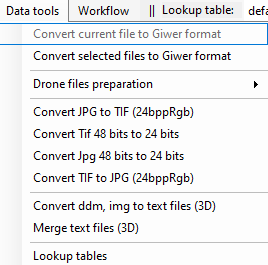
\includegraphics[width=6cm]{datatools_menu.png}
		\caption{A \textit{Data tools} menü}
		\label{fig:datatools_menu}
	\end{figure}



A \textit{Convert to Giwer format} menü csak akkor aktív, ha a \textit{Layers} fül listáján valamely tif, jpg vagy bil formátumban lévő kép ki van választva. Erre a menüre kattintva végrehajtódik a konverzió, és a \textit{Config} fájlban megadott helyre (GiwerDataFolder) képződik a konvertált adat. Ezután ezt a fájlt megnyitva a \textit{Data Stock} teljes funkcionalitása rendelkezésre áll. A többi formátumú kép számára a feldolgozó műveletek nem aktivizálhatók, csak a \textit{giwer} formátumúakra.

A \textit{Convert selected files to Giwer format} menüt akkor érdemes használni, ha egyszerre sok fájlt akarunk konvertálni. A menüre kattintva kiválaszthatjuk a fájlokat, és a konverzió végrehajtódik az össze fájlra.

A \textit{Drone files preparation} menü bizonyos képek \textit{gwr} formátumba hozására szolgál. A Micasense multispektrális kamera, amelyeknek három RGB, és két infravörös sávja, valamint egy termális sávja van, annyi tif fájlt állít elő, ahány sávja van, jelen esetben 6 db tif fájlt. Ha ezeket szeretnénk gwr formátumba konvertálni, akkor két lehetőségünk van, amit két almenü tesz lehetővé:
\begin{itemize}
	\item A \textit{Merge multiple images to giwer format} menüre kattintva megjelenik egy dialógus ablak, ahol kiválaszthatjuk a kérdéses fájlokat. Ezután elindul a konverziós folyamat, amelynek eredményeként egy db \textit{GWH} fájl és 6 db \textit{GWR} fájl keletkezik. A header egy 6 sávos képet fog leírni. Mindenképpen ez a módszer ajánlható, mert a \textit{Multiband processes} feldolgozási folyamatok csak ilyen fájlokra működnek.
	
	\item A \textit{Convert each multiple image to giwer format} menüre kattintva megjelenik egy dialógus ablak, ahol kiválaszthatjuk a kérdéses fájlokat. Ezután elindul a konverziós folyamat, amelynek eredményeként 6 db \textit{GWH} fájl és 6 db \textit{GWR} fájl keletkezik. Így minden egyes sáv egysávos képnek fog látszani. Ezekre csak a \textit{One band processes} menü funkciók fognak működni.
\end{itemize}

A \textit{Convert ddm, img to text files(3D)} menü bináris domborzatmodell fájlokból text fájlt készít (soronként xyz adatokkal). Ennek akkor vesszük hasznát, ha a későbbiekben olyan domborzat elemző programot is szeretnénk használni, amely nem olvassa a konkrét bináris fájlt. A 3D-s text fájl ugyan nagy méretű, de minden 3D-s program képes beolvasni.

A \textit{Merge text files(3D)} menüre kattintva egyesíthetünk text formátumú domborzat modelleket egyetlen 3D-s text fájllá.

A \textit{Workflow} menüre kattintva elindul a \textit{WorkflowBuilder}, ami amúgy a keretprogramból is indítható.

\subsection{Ikonosztáz}

A főbb funkciócsoportok után néhány apróbb, inkább kényelmi funkciót is ismertetünk. A menüsor alatt található egy ikonosztáz, amely a menürendszerből bizonyos funkciókat gyorsabban elérhetővé tesz:\\

\includegraphics[height=0.55cm]{ikonosztaz.png} \\Balról jobbra a következő funkciók érhetők el: gwr(G), bil(B), tif(T), jpg(J), 3D (\includegraphics[height=0.55cm]{3dikon.png}) és videó fájlok megnyitása, RGB (
\includegraphics[height=0.55cm]{rgbikon}) kép készítése, kétféle hisztogram művelet, ahol az első (
\includegraphics[height=0.55cm]{histo1ikon}) interaktív, és meg is jeleníti a hisztogramot, a másik automatikus (
\includegraphics[height=0.55cm]{histo2ikon}). Cross plot rajzoló (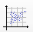
\includegraphics[height=0.55cm]{cpikon}) két frekvenciasáv adatait jeleníti meg egy grafikonon, ahol ahol grafikus is szelektálhatunk a pixelek között. A 
\includegraphics[height=0.55cm]{headerikon} ikon a header adatok elrejtését/megjelenítését végzi. 

A 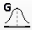
\includegraphics[height=0.55cm]{gaussikon} ikon Gauss-simítást, a 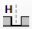
\includegraphics[height=0.55cm]{highpassikon} a high pass filtert indítja, az 
\includegraphics[height=0.55cm]{medianikon} a medián szűrést, az 
\includegraphics[height=0.55cm]{laplaceikon} a Laplace szűrést, a 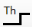
\includegraphics[height=0.55cm]{thresholdikon} a thresholdingot. Ezután jön az osztályozás ikonja (
\includegraphics[height=0.55cm]{clusterikon}), majd az NDVI számítóé (
\includegraphics[height=0.55cm]{ndviikon}), a főkomponens analízisé (
\includegraphics[height=0.55cm]{pcaikon}), majd a raszter kalkulátor (
\includegraphics[height=0.55cm]{calcikon}), és végül a lookup table szerkesztő (
\includegraphics[height=0.55cm]{lookupikon}). A 
\includegraphics[height=0.55cm]{undoikon} ikon az \textit{undo} funkció, vagyis visszaállítja az utolsó művelet előtti állapotot (csak egy visszalépés lehetséges). 

A \textit{Layers} fülön három ikon van: 
\includegraphics[height=0.55cm]{layer_list_icons.png}. A piros kereszt törli az egész layer listát. A kinyíló könyv az összes listán lévő kép frekvenciasávjainak listáját kinyitja, míg a bezáródó könyv bezárja őket. 

Egyenként is törölhetünk is a listáról, de csak a fájlcsoportokat, az egyes sávokat nem. Ha tehát le szeretnénk törölni egy fájlcsoportot, akkor a jobb egérgombbal klikkeljünk a kívánt elemre, és a felbukkanó menüből válasszuk ki a törlést.

Ha valamelyik sávra a jobb egérgombbal kattintunk, akkor lehetőségünk van egy külön ablakban megjeleníteni azt.

\subsubsection{Layerlist, Header, Exif, Project description}

A gyors menüből a 
\includegraphics[height=0.55cm]{headerikon}-ra kattintva ki/be kapcsolatható a bal oldali metaadatokat mutató sáv. A \textit{Layers} fül a réteglistát mutatja meg. A \textit{Header} fülre kattintva megnézhetjük az éppen aktuális kép header adatait (\ref{fig:header}. ábra). 

	\begin{figure}
	\centering
	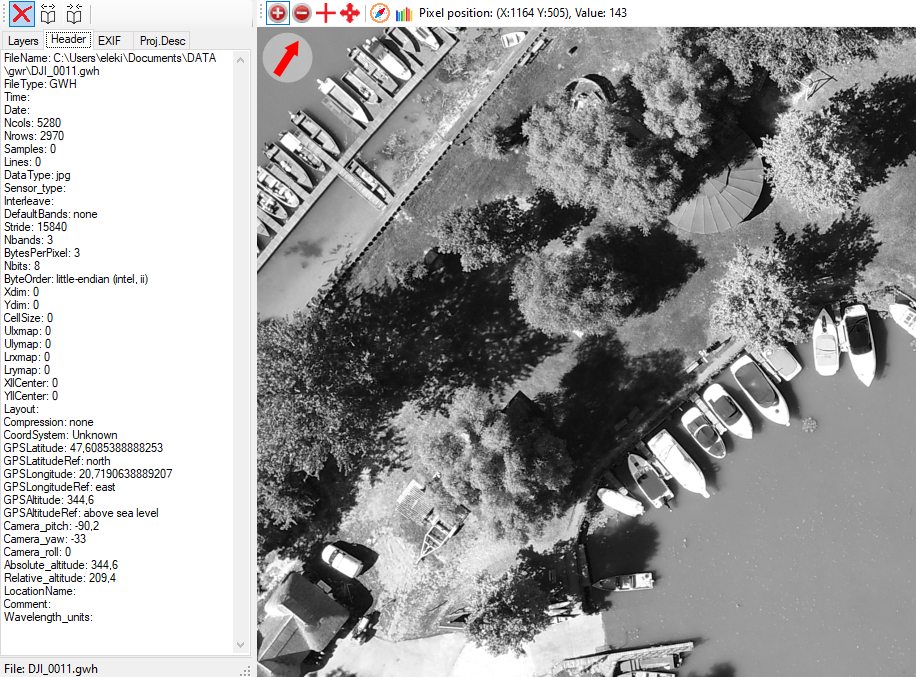
\includegraphics[width=12.5cm]{header}
	\caption{A header. Üres mezők is láthatók, amely azt jelenti, hogy ezek nem relevánsak az adott képre nézve, vagy nem állnak rendelkezésre}
	\label{fig:header}
	\end{figure}



Ha a header területére bárhová kattintunk, szerkeszthetővé válik a header, persze csak azok az adatok, amelyek írhatók. Az \textit{Exif} fülre kattintással megjelennek az exif adatok (ha vannak ilyenek, mert ilyesmi csak \textit{tif} és \textit{jpg} adatoknak van). A \textit{Proj.Desc} fülre klikkelve megjelennek a projekt leíró adatai, ha vannak ilyenek. Ha szeretnénk a megnyitott képeket projektbe szervezve menteni, akkor ide beírhatjuk a projekt leírását.

\subsection{Megjelenítő}

Amikor a réteglistán kijelölünk egy frekvenciasávot, akkor annak megjelenik a képe. Ahogy mozog a kurzor az ablakban, úgy látjuk az éppen aktuális pixel pozícióját és intenzitás értékét. A nagyító ikonra klikkelve (
\includegraphics[height=0.55cm]{magnifyikon}) nagyítás üzemmódba kerül az ablak. Tetszőleges területet jelölhetünk ki a nagyításra. Ennek az ellenkezője, a zoom out funkció akkor hajtódik végre, amikor a 
\includegraphics[height=0.55cm]{zoomoutikon} ikonra kattintunk. A 
\includegraphics[height=0.55cm]{panikon} ikonra kattintva pan üzemmódba kerülünk. Ha ilyenkor a képen valahová klikkelünk, akkor a kép úgy fog eltolódni (változatlan nagyítás mellett), hogy a kép közepe a klikkelés helyére fog kerülni. A 
\includegraphics[height=0.55cm]{zoomfullikon} ikonra kattintva a kép teljes egészében meg fog jelenni.

Ha ráklikkelünk a 
\includegraphics[height=0.55cm]{compassikon} ikonra, akkor a kép bal felső sarkában megjelenik az északi irányt mutató nyíl (feltéve, hogy a kép leíró adataiból ez megállapítható). Ha a 
\includegraphics[height=0.55cm]{spektrumikon} ikonra kattintunk, akkor spektrum néző üzemmódba kerülünk. Ha bárhova klikkelünk a képen a bal egérgombbal, akkor az adott pixel spektruma fog megjelenni az ablak jobb oldalán grafikusan és táblázatos formában. Ha jobb oldali egérgombbal klikkelünk, akkor ahogy mozog a kurzor, úgy láthatjuk a pixelről pixelre változó spektrumot.

A \ref{fig:spektrum_compass}. ábrán egy hiperspektrális képet láthatunk az iránytűvel és a az egyik pixelhez tartozó spektrummal.

	\begin{figure}
	\centering
	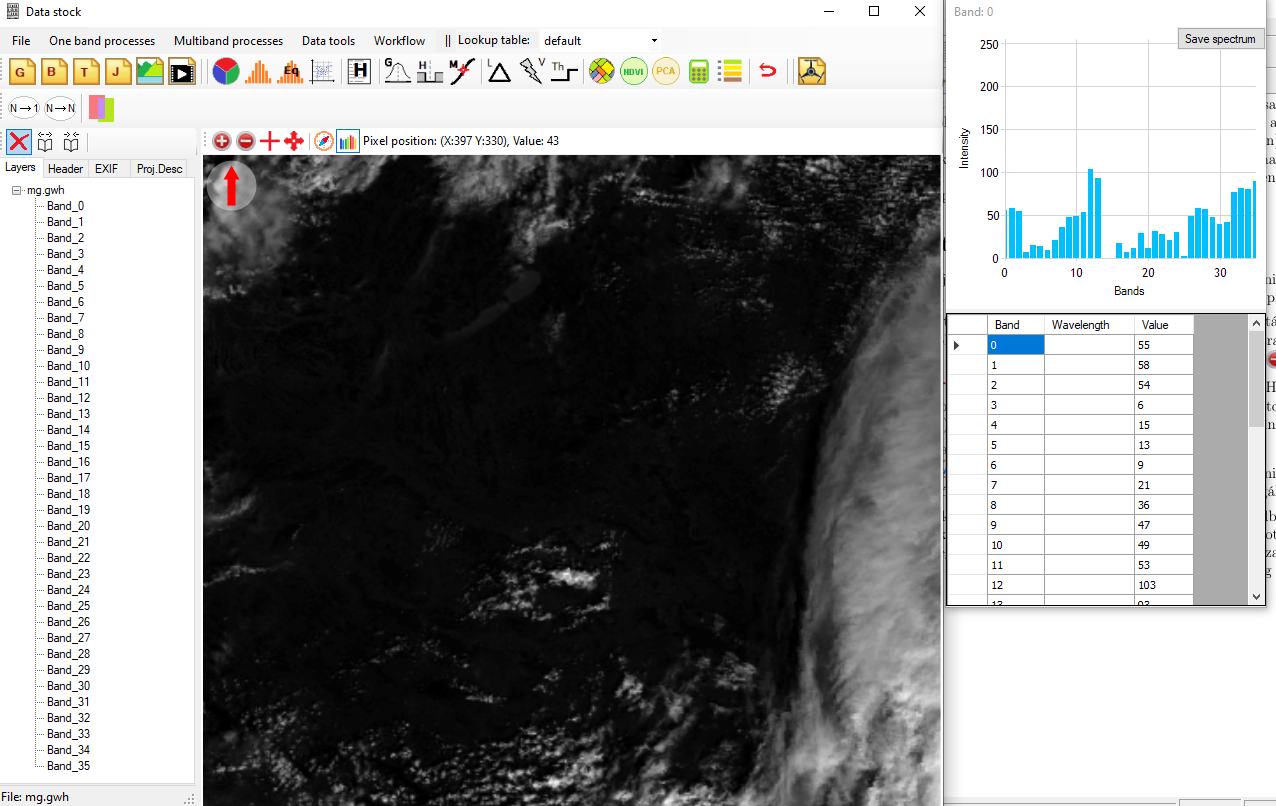
\includegraphics[width=13cm]{spect_compass}
	\caption{Egy hiperspektrális kép (37 sávos) az iránytűvel és egy pixel spektrumával}
	\label{fig:spektrum_compass}
	\end{figure}


%\includegraphics[height=0.55cm]{}
\subsubsection{Példák}

A fentebb leírt függvényekből bemutatunk néhányat:

	\begin{figure}
	\centering
	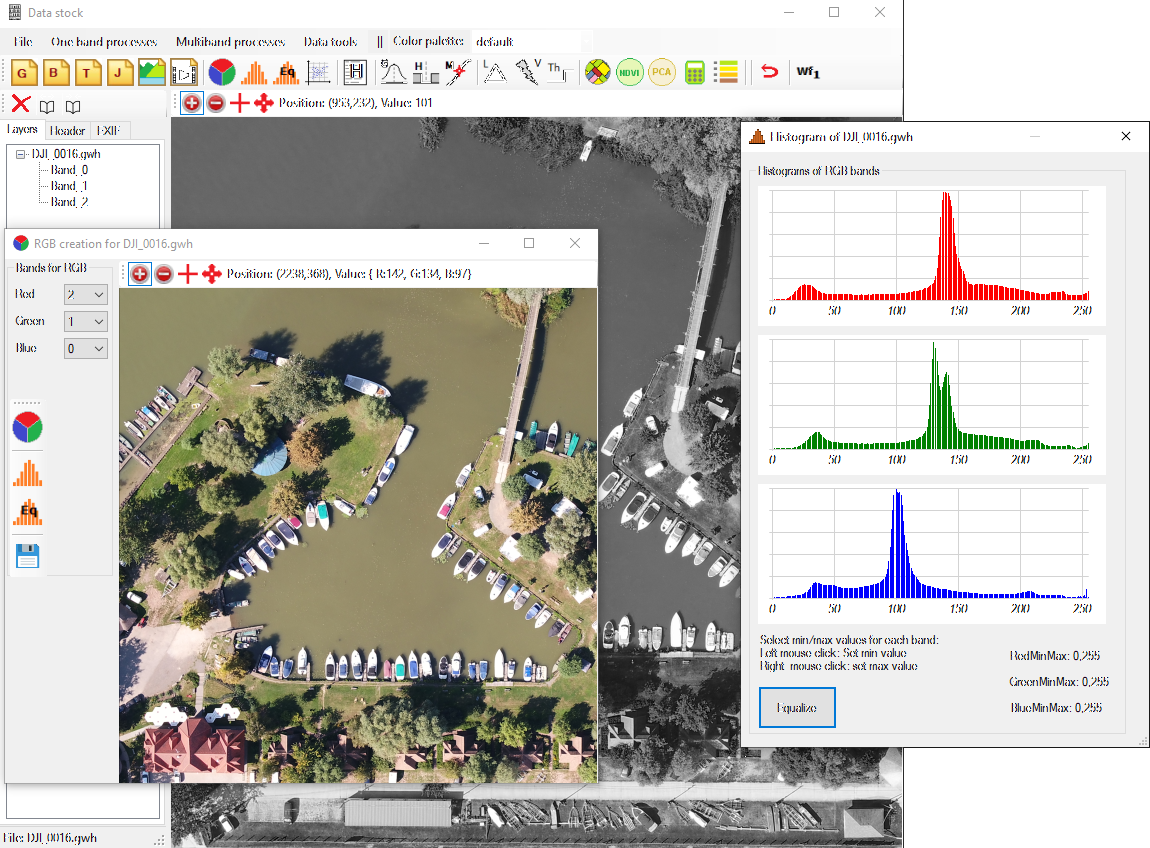
\includegraphics[width=12cm]{gw1.png}
	\caption{Greyscale, RGB and histogram ablak}
	\label{fig:gw1}
\end{figure}

\begin{figure}
	\centering
	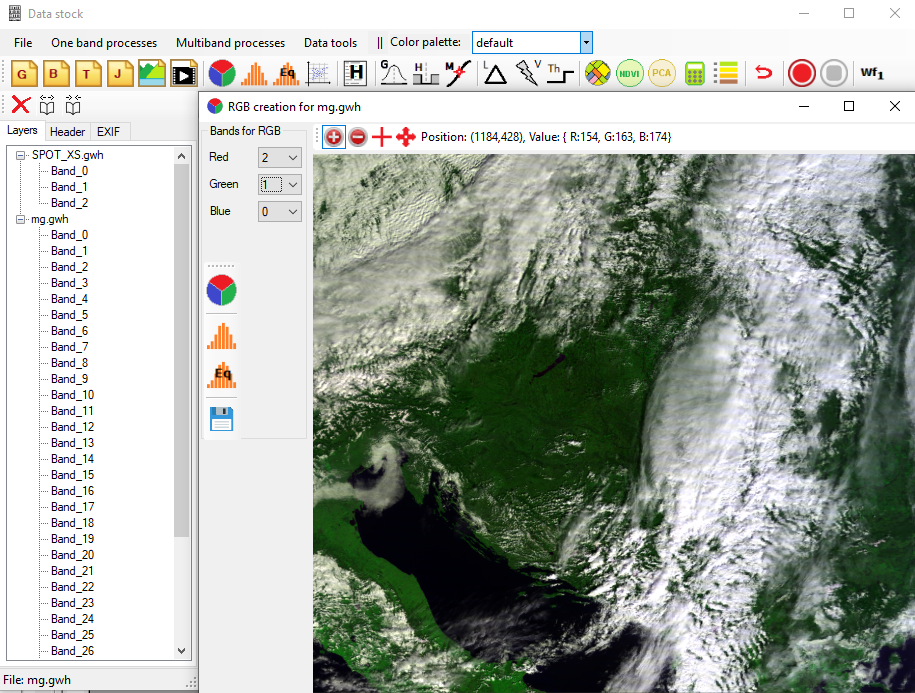
\includegraphics[width=12cm]{ds1.png}
	\caption{RGB ablak egy hyperspectral képről}
	\label{fig:ds1}
\end{figure}

\begin{figure}
	\centering
	
\includegraphics[width=12cm]{ndvi.png}
	\caption{RGB versus NDVI}
	\label{fig:ndvi}
\end{figure}

\begin{figure}
	\centering
	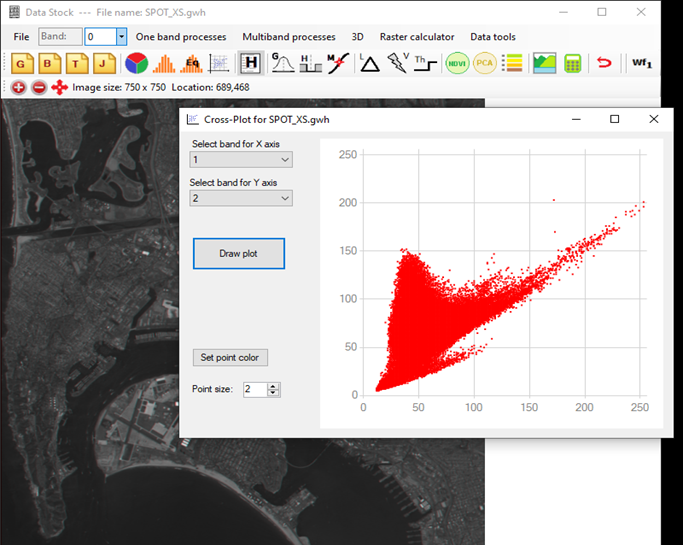
\includegraphics[width=12cm]{crossplot.png}
	\caption{Crossplot: green band versus red band}
	\label{fig:crossplot}
\end{figure}

\begin{figure}
	\centering
	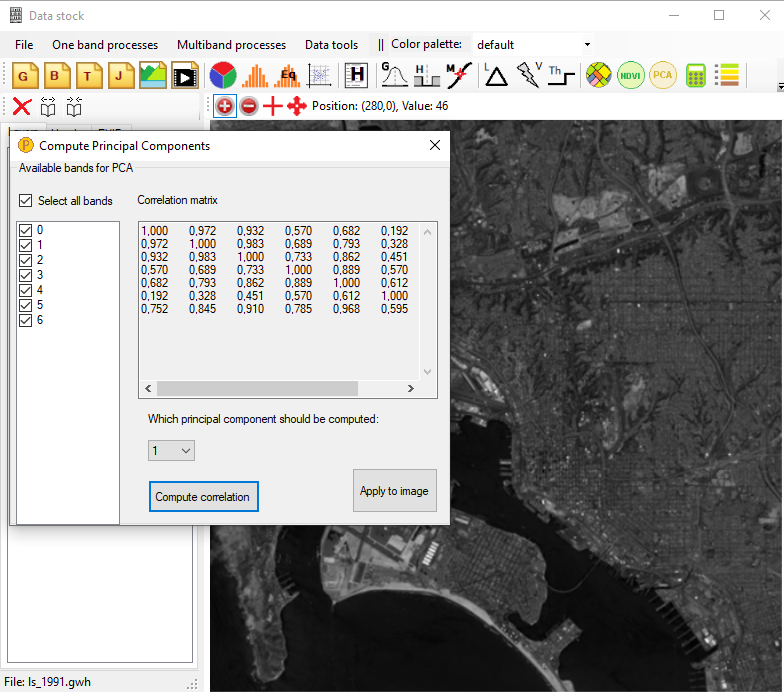
\includegraphics[width=12cm]{pca2.png}
	\caption{A korrelációs mátrix és az első főkomponens egy Landsat képre}
	\label{fig:pca2}
\end{figure}

\begin{figure}
	\centering
	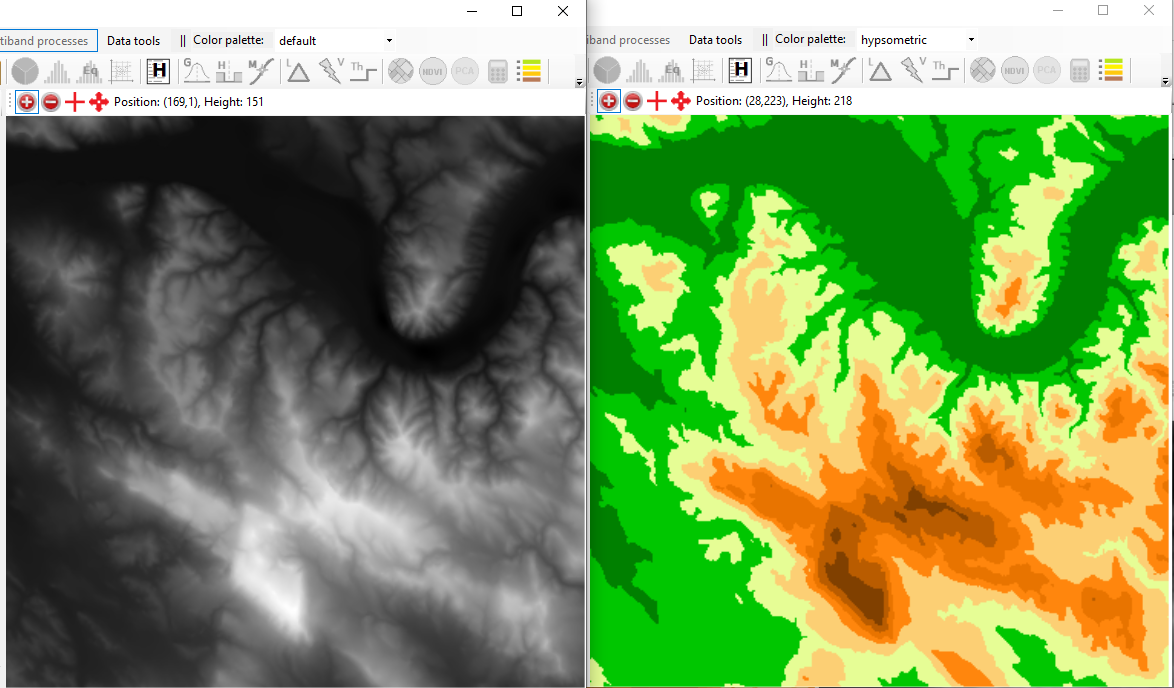
\includegraphics[width=12cm]{dtm.png}
	\caption{Digital terrain modell a Dunakanyarra (greyscale és hypsometric shading)}
	\label{fig:dtm}
\end{figure}

\begin{figure}
	\centering
	
\includegraphics[width=9cm]{cluster.png}
	\caption{A klaszterezés eredménye}
	\label{fig:cluster}
\end{figure}

\begin{figure}
	\centering
	\includegraphics[width=9cm]{cloud.png}
	\caption{Példa egy workflow eredményéről: pontfelhő határ detektálás}
	\label{fig:cloud}
\end{figure}

\begin{figure}
	\centering
	\includegraphics[width=10cm]{rastcalc.png}
	\caption{Raszter kalkulátor ablak}
	\label{fig:rastcalc}
\end{figure}

\begin{figure}
	\centering
	\includegraphics[width=10cm]{lut.png}
	\caption{View/edit lookup table és a colour palette}
	\label{fig:lut}
\end{figure}

\begin{figure}
	\centering
	\includegraphics[width=14cm]{aligning.png}
	\caption{Korrigált Micasense kép (jobb oldali ábra), korrekció előtti (bal oldali ábra)}
	\label{fig:aligning}
\end{figure}



\section{Catalog}

A \textbf{Catalog} alrendszer nagy tömegben keletkező képek (csak \textit{jpg} és \textit{tif} formátumú képek) rendszerezésére, adatbázisba szervezésére való (ehhez sqlite-ot használ a program). Az adatok és a képek gyors szemrevételezését is lehetővé teszi. A \textbf{DataStock} alrendszer használata enélkül is lehetséges, hiszen bármely képet használatba vehetjük vele. A \textbf{Catalog}ot olyankor célszerű használni, amikor több száz vagy több ezer képet kívánunk egységesen kezelni, a leíró adataik alapján keresést végezni.

\subsection{Első lépések}

\begin{itemize}
	\item Másoljuk be egy könyvtárba a catalog.zip fájlt.
	\item Bontsuk ki.
	\item Ahová kibontottuk, onnan indítható a catalog.exe, nem kell külön telepíteni.
	\item Az első induláskor még nincs képi adatbázis, ezért panaszkodni fog a hiányára (\ref{fig:missingdb}. ábra):
	
	\begin{figure}[h]
		\centering
		\includegraphics[width=8cm]{missingdb.png}
		\caption{A 'Missing database' üzenet}
		\label{fig:missingdb}
	\end{figure}
	
	\item Ezután megjelenik a program fő formja, ahol kreálhatunk egy új, üres adatfájl (\ref{fig:createnewcatalog}. ábra) (a default név 'dronimagecatalog.s3db', de lehet bármi más is)
	
	\begin{figure}
		\centering
		\includegraphics[width=8cm]{createnewcatalog.png}
		\caption{A \textit{Create new catalog} menü}
		\label{fig:createnewcatalog}
	\end{figure}
	
	\item Ezután a 'Open' menüre klikkelve megnyílik az üres adatbázis-fájl.
	
	\item Ha már van létező adatbázis (pl. dronimagecatalog néven), akkor megjelenik a tartalma egy táblázatban a program fő formján (\ref{fig:catalog0}. ábra). Ritka eset, de ha nincs, akkor panaszkodni fog, hogy nincs ilyen adatbázis  –- mert például kitörültük a fájlrendszerből, de a catalog még úgy emlékszik, hogy van ilyen fájl. Kattintsunk az OK-ra, majd nyomjuk meg az F2 gombot -– bal felső sarok környéke a billentyűzeten. Ekkor megjelenik egy 'Catalog' nevű menü. Válasszuk ki a 'Create new catalog' almenüt, amely létrehoz egy 'dronimagecatalog' nevű adatbázist, és benne egy üres adattáblát, amelynek 'images' lesz a neve. Ide fognak képződni a felvett képek adatai.
	
	\begin{figure}
		\centering
		\includegraphics[width=13cm]{catalog0.png}
		\caption{A \textit{Catalog} fő formja}
		\label{fig:catalog0}
	\end{figure}
	
	\item Normál indulásnál a menürendszer nem látszik (F2-t megnyomva jelenik meg és tűnik el)
	
	\item Az ikonok elmondják, hogy mit tudnak, ha az egeret föléjük mozgatjuk.
	
\end{itemize}

\subsection{A fájlrendszer előkészítése}

\begin{itemize}
	\item Kreáljunk egy könyvtárat 'DRON\_IMAGES' néven valahol a fájlrendszerben.
	
	\item Klikkeljünk az 'open folder tree' ikonra (\includegraphics{open_folder_structure.png}). Ekkor megnyílik a 'Folder structure' nevű ablak (\ref{fig:folder_struc}. ábra).
	
	\item Klikkeljünk a 'Set destination folder' nevű menü gombra, majd keressük meg és válasszuk ki a 'DRON\_IMAGES' nevű könyvtárat. Ezzel megadtuk a kép katalógus helyét a fájlrendszerben, amire ezentúl emlékezni fog a program, ha újra megnyitjuk a 'Folder structure' ablakot. 
	
	\item Keressük meg a flash driven-on (ami a dronon a képeket tárolja) azt a könyvtárat, ahol az éppen most készített képek vannak. Ha a jobb oldali ablakban megjelennek a fájlok, klikkeljünk a 'Save files to '\verb|c:\DRON_IMAGES| folder' ikonra (\includegraphics{save.png}). Ennek hatására az egész könyvtár tartalma átmásolódik a flash driveról a 'DRON\_IMAGES' nevű könyvtárba.
	
	\item Ennek hatására a 'DRON\_IMAGES' nevű könyvtárban megjelenik egy új directory, aminek a neve az első fájl mentésének időpontja. Ez a könyvtár fogja tartalmazni az adott időben történt repülés képeit.
\end{itemize}

\begin{figure}
	\centering
	\includegraphics[width=13cm]{folder_struc.png}
	\caption{A \textit{Folder structure} ablak}
	\label{fig:folder_struc}
\end{figure}

\subsection{A Micasense kamera képeinek korrekciója}

A Micasense kamera képalkotási hibáit korrigálni kell, mielőtt használatba vennénk. Mivel minden frekvenciasáv képe egy különálló kamerával készült, így ezek képei között kisebb nagyobb elcsúszások vannak. Enélkül a multispektrális képek használhatatlanok.

\begin{figure}
	\centering
	\includegraphics[width=11cm]{mica_aligned}
	\caption{A korrigált (aligned) képekből készült RGB, amely a vörös és a két infravörös sávból készült}
	\label{fig:mica_aligned}
\end{figure}

A korrekciót a \includegraphics[width=0.5 cm]{aligner} ikonra kattintva indíthatjuk el. Megnyílik egy fájl dialógus ablak, ahol kiválaszthatjuk a kép fájlokat. Ne felejtsük el, hogy a Micasense annyi kép fájlt készít, ahány sávos a kamera (vagyis 5+1). Az első öt fájl három RGB plusz két infravörös sáv. A hatodik egy termál sáv, amely sokkal rosszabb felbontású, mint a több fájl. Ezt ne vegyük be a kép sávjainak összeigazításába. A \ref{fig:mica_aligned}. ábrán a korrigált kép látható.



\subsection{Az adatbázis feltöltése}

\begin{itemize}
	\item Kétféleképpen tölthetjük fel az adatbázist: vagy egyenként (vagy multiselecttel több fájlt is) vagy egy directory-t kijelölve tömegesen, annak teljes tartalmát (csak jpg és tif fájl, más nem). A fájlonkénti kijelöléshez klikkeljünk a sárga plusz jelre (\includegraphics[width=0.5cm]{plus.png}), a teljes directory kijelöléséhez a zöld karikában fehér kereszt ikonra (\includegraphics[width=0.5cm]{addfolder.png}).
	
	\item Bármelyikre klikkeltünk, felbukkan a 'Editable image attributes' nevű ablak (\ref{fig:editableimageattribute}. ábra), ahol megadhatjuk azokat az adatokat, amelyek minden most beemelendő képre vonatkoznak. A többi adatot a program automatikus feltölti (fájlnév, long, lat, timestamp, folder, stb.).
	
	\begin{figure}
		\centering
		\includegraphics[width=6cm]{editableimageattributes.png}
		\caption{Az \textit{Editable image attributes} ablak}
		\label{fig:editableimageattribute}
	\end{figure}
	
	\item A táblázat nem automatikus adatai szerkeszthetők, amik el is mentődnek, amint a következő rekordra lépünk.
	
	\item A fényképezőgép ikonra \includegraphics[width = 0.5 cm]{camera.png}) kattintva megjelenik az aktuális rekordhoz tartózó kép. Az 'Exif' (\includegraphics[width = 0.6 cm]{exif.png}) feliratú ikon az aktuális rekordhoz tartozó kép exif adatait mutatja meg egy külön ablakban.
\end{itemize}

\subsection{Funkciók}

Az adatokat mutató táblázat felett egy ikonosztáz látható, amelyen a főbb funkciók lettek elhelyezve. A \includegraphics[width = 0.5 cm]{filesystem.png} ikon megnyit egy a fájlrendszert nézegető ablakot, hol megnézhetjük az adatok forrását, mint pl. egy pendrive-ot, ami közvetlenül a drón adattároló eszköze, és amelyen a legfrissebb mérési adatok vannak(\ref{fig:folder_struc}. ábra). A kiválasztott fájlokat (az egész könyvtárat) a \textit{DRON\_IMAGES} nevű könyvtárba másolja be. Amúgy ezt az első használat során meg kell adni (\textit{Set destination folder}). A másolást a \includegraphics[width=0.5cm]{save.png} ikonra való klikkelés végzi.

Az adatbázisban már bent lévő képeket a \includegraphics[width = 0.5 cm]{camera.png}  ikonnal, míg a hozzá tartozó EXIF adatokat az \includegraphics[width = 0.5 cm]{exif.png}  ikonnal nézhetjük meg.

Új képeket, egyenként a \includegraphics[width=0.5cm]{plus.png} ikonnal, míg tömegesen, vagyis egy egész directory tartalmát, a \includegraphics[width=0.5cm]{addfolder.png} ikonnal adhatjuk hozzá az adatbázishoz. A hozzáadás egyben az adatbázis feltöltését is elvégzi, persze csak azokat az adatokat, amelyek a képekből kinyerhetők. Interaktívan is hozzáadhatók adatok, ha azokat a megfelelő mezőbe beírjuk. A \includegraphics[width=0.5cm]{del.png} ikonnal egy kijelölt rekordot törölhetünk. Nemcsak a leíró adatok törlődnek (az 'images' nevű tábla kijelölt rekordja), hanem a \textit{DRON\_IMAGES} könyvtárból is a kijelölt kép fájl (UNDO nincs!).

\begin{figure}[h]
	\centering
	\includegraphics[width=12cm]{sqleditor.png}
	\caption{Az \textit{Sql editor} ablak}
	\label{fig:sqleditor}
\end{figure}

Az \includegraphics[width=0.5cm]{sql.png} ikonnal SQL parancsokat állíthatunk össze, amelyekkel tetszőleges feltétel szerint kereshetünk (legyűjthetünk) a rendelkezésre álló képek paraméterei alapján. Az \ref{fig:sqleditor}. ábrán olyan képek legyűjtésének eredménye látható, amelyek a Tiszán készültek, és a kép típusa 'multispektrális'. Az 'Sql editor' az Sql-t nem, vagy csak alapszinten ismerők számára is használható. 
(Az Sql-ben járatos felhasználók számára előhívható egy rejtett Sql parancssor, amely azért rejtett, mert hozzá nem értők kezében veszélyes fegyver lehet, amellyel súlyos károkat is lehet okozni az adatbázisban. Akik biztosak az Sql tudásukban, azok az F12 gomb megnyomásával előhívhatják az Sql parancssort, amely eltüntethető, ha újra megnyomjuk az F12 gombot. Nemcsak lekérdező, hanem non query típusú parancsok is kiadhatók. A parancs \textbf{Enter}rel hajtható végre.)


A \includegraphics[width = 0.5 cm]{sheet.png} ikonnal egy adott mérésre vonatkozó riport fájlt nézhetünk meg, vagy hozhatunk létre, amelybe olyan adatokat tehetünk bele, amelyeket a mérési körülmények miatt, vagy bármilyen szempontból érdekesnek találunk, de nem az egyes képekhez kötöttek.

\subsection{Lekérdezés}

	\begin{figure}
	\centering
	\includegraphics[width=12cm]{mapviewer_select_all.png}
	\caption{A \textit{Map viewer} ablak}
	\label{fig:mapviewer_select_all}
\end{figure}

\begin{figure}
	\centering
	\includegraphics[width=12cm]{mapviewer.png}
	\includegraphics[width=12cm]{tegeta.png}		
	\caption{A \textit{Map viewer} ablak. Felső részen a Kormorán kikötő (Tiszafüred), míg az alsón az ELTE látható}
	\label{fig:mapviewer}
\end{figure}

\begin{itemize}
	\item  Az 'SQL' feliratú ikonra klikkelve (\includegraphics[width=0.5cm]{sql.png}) megjelenik egy 'Query editor' nevű ablak. Itt ki lehet választani, hogy melyik mezőre kérdezünk, milyen feltételt szabunk.
	
	\item pl. select field: type;  Operator: =; Value: RGB $\rightarrow$ 
	WHERE type=RGB. Ha itt vége, akkor click to 'Generate WHERE condition and Sql command' majd 'Execute query'. 
	
	\item Ha új lekérdezés lesz, akkor előtte click to 'Clear WHERE or new command'. Vigyázat, az Sql editor case sensitive (rgb !=  RGB)
	
	\item Összetettebb lekérdezésekhez az előbbihez hasonló lekérdezés után klikkeljünk az 'Add further condition' nevű check boxra. 
	
	\item Ha kész vagyunk egy further feltétellel, klikkeljünk az 'Add further condition'- gombra. Ha az utolsót is hozzáadtuk, akkor klikkeljünk a 'Generate WHERE condition and Sql command' majd az 'Execute query'-re. Ha jó volt az sql parancs, akkor megjelenik az eredmény az adatrácsban.
	
	\item Ha meg vagyunk elégedve az eredménnyel, klikkeljünk a 'Close and return to main window' gombra. Ekkor becsukódik a 'Query editor' ablak, és a lekérdezés eredménye megjelenik a fő ablakban. Itt nézegethetjük a képek listáját.
	
	\item A 'Select all' feliratú gombra a bal egérgombbal klikkelve az összes képet legyűjthetjük az adatbázisból, amelyek adatai meg is jelennek az adatrácsban.
	
	\item A 'Select all' feliratú gombra a jobb egérgombbal klikkelve az összes képet kijelölhetjük az  adatrácsban (\ref{fig:mapviewer_select_all}. ábra). Ez olyankor hasznos, amikor térképen akarjuk megjeleníteni a legyűjtött képek centroidjait. Ehhez még rá kell kattintani a \includegraphics[width = 0.5 cm]{mapviewer_ikon.png} ikonra. Ekkor megjelennek a 'Map viewer' ablakban (\ref{fig:mapviewer}. ábra felső része) a képek centroidjai. Ha úgy klikkeltünk a \includegraphics[width = 0.5 cm]{mapviewer_ikon.png} ikonra, hogy nem jelöltünk ki egyetlen képet sem, akkor az ELTE Térképtudományi és Geoinformatikai Intézet helye jelenik meg a térképen (a \ref{fig:mapviewer}. ábra alsó része).
	
	
	
	\item Sql-ben járatos felhasználóknak közvetlen Sql parancssor is rendelkezésre áll. Ha megnyomjuk az F12 gombot, akkor megjelenik a parancssor. Újból megnyomva eltűnik. Ezt csak biztos tudású SQL szakértő használja, mert nincs UNDO. Igaz, hogy ha elfelejtettük a képek adatbázisba beemelésekor megadni az összes új képre vonatkozó interaktív mező tartalmát, akkor már csak itt tudunk tömeges értékadás végrehajtani (UPDATE), feltéve, hogy meg tudjuk egymástól különböztetni az új képek rekordjait a többitől.
	
	
	
\end{itemize}


\section{Workflow builder}

A \textbf{Giwer}-ben igen sok funkciót implementáltunk, melyeket a \textbf{DataStock} modulban a menürendszeren keresztül érhetünk el. Interaktívan dolgozhatunk, egy-egy fájlon mindenféle eljárást kombinálva juthatunk el kívánt eredményig. 

Amikor azonban több száz kép vár feldolgozásra, akkor ez az egyenkénti feldolgozási mód meglehetősen hosszadalmas és fáradságos munka. Egy-egy terület megismerésével, amit néhány kép interaktív feldolgozásával értünk el, megfogalmazhatunk olyan, a területre általános érvényű feldolgozási módszertant, amit jó lenne az összes képre alkalmazni. Erre a feladatkörre dolgoztuk ki a \textbf{Workflow builder}t.

Az implementált függvények közül nem mindegyik való végfelhasználó kezébe, mert valami olyasmit csinál, amit a felhasználó nem használna önállóan (pl. konverzió bitmapből bytetömbbe), de a rendszernek szüksége van rá. Vannak azonban olyan eljárások (szűrők, osztályozók, NDVI, PCA), amire viszont szükség lehet egy feldolgozási folyamat összeállításakor. Ezért összegyűjtöttük ezeket a függvényeket, és a \textbf{workflow builder}ben felajánljuk egy listán a végfelhasználónak. Ezek közül választva összeállíthatja a saját munkafolyamatát, amit elmenthet és futtathat.

\subsection{Használat}

A modult vagy a keretrendszerből indíthatjuk el a \textbf{Workflow builder} feliratú gombbal, vagy a DataStock modul \textit{Workflow} menüpontjára klikkelve aktivizálhatjuk. Elindítás után megjelenik a fő ablak (\ref{fig:workflowmain}. ábra).

	\begin{figure}      
	\centering
	\includegraphics[width=12cm]{workflow_main}
	\caption{A \textit{Workflow Builder} ablak}
	\label{fig:workflowmain} 
    \end{figure}

Az ablak bal oldalán látható az \textit{Operations} feliratú lista, amely az elérhető függvények neveit mutatja. Ebből választhatunk vagy dupla klikkeléssel vagy a megjelölt listaelem után a \includegraphics[width=0.4 cm]{zoldplus} jelre klikkeléssel. Ekkor átkerül a kiválasztott eljárás neve a jobb oldali listára. Annyi eljárást tehetünk ide, amennyi csak szükséges.

Mivel az eljárásoknak vannak paraméterei, ezért ezeket úgy adhatjuk meg, ha ráklikkelünk a kiválasztott eljárásra. Ekkor a \textit{Parameteres} ablakban megjelennek a megadandó paraméterek nevei és egy szöveg doboz, ahol megadhatjuk ezeket az értékeket. Az \textbf{Enter} leütésével fogadjuk el a begépelt értéket. \textbf{Enter} nélkül nem jegyzi meg.

\subsubsection{Menürendszer}

A menürendszer igen egyszerű. A \textit{File} menü elemeit mutatja a \ref{fig:workflowmenu}. ábra. A \textit{Create new workflow}-val új workflowt hozhatunk létre. Ilyenkor az elérhető eljárások listáját tartalmazó lista kivétel minden törölve lesz. Új eljárás esetén ki kell tölteni a \textit{Name} mezőt, amely a workflow mentéskori nevét hivatott megadni. A workflow fájlok kiterjesztése \textit{wkf}.

Ne hagyjuk üresen a \textit{Description} mezőt, mert később hasznos lehet az ide írt információ. Ha minden paramétert is adatot beírtunk, akkor kattintsunk a \textit{Save workflow} almenüre. Ezzel elmentettük a megadott helyre, ahonnan bármikor visszaolvasható és szerkeszthető.

Ha egy meglévő workflowt szeretnénk használni, kattintsunk a \textit{Load workflow} almenüre. Ekkor megjelennek a wokflow neve, leírása és a kiválasztott függvények nevei. 
Ha valamely workflow feleslegessé válik, kitörölhetjük a \textit{Delete workflow} menüre kattintással.

	\begin{figure}
	\centering
	\includegraphics[width=4.5cm]{workflow_menu}
	\caption{A \textit{Workflow Builder} menüi}
	\label{fig:workflowmenu}
	\end{figure}

A \ref{fig:workflowfile} ábra egy workflow fájlt mutat. Ez is egy egyszerű szövegfájl, de a projekt fájlhoz hasonlóan ezt sem célszerű "kézzel" editálgatni, mert könnyű elrontani, és akkor használhatatlanná válhat a workflow. Nem a végfelhasználónak készült, hanem a rendszernek.

	\begin{figure}[h]
	\centering
	\includegraphics[width=9cm]{workflowfile}
	\caption{Példa egy egyszerű workflow fájlra. A függvény neve után zárójelben látható, hogy hány paramétert vár az eljárás}
	\label{fig:workflowfile}
	\end{figure}


\subsubsection{Ikonosztáz}

A \includegraphics[width=0.4 cm]{zoldplus} ikont már ismerjük. Ezzel választhatjuk ki a workflowba beemelni kívánt függvényeket az \textit{Operations} nevű listáról.
Ha egy függvény feleslegessé vált egy worklowban, akkor a \includegraphics[width=0.4 cm]{pirosminus} ikonra kattintással lehet levenni a listáról.
A lista elemeit a \includegraphics[width=0.4 cm]{nyilfel} és \includegraphics[width=0.4 cm]{nyille} nyilakkal tudjuk fel-le mozgatni, ami azért lényeges, mert a workflow a lista sorrendjének megfelelően hajtja végre a műveleteket.
A \includegraphics[width=0.4 cm]{saveworkflow} ikonnal elmenthetjük a workflow fájlt, ami az eljárások nevei mellett a szükséges paraméterek értékeit is tartalmazza. Mentés nélkül nem futtatható a workflow.
A futtatást a \includegraphics[width=0.4 cm]{runworkflow} ikon indítja.

Amíg nem adtunk nevet a workflownak, addig passzív marad a \includegraphics[width=0.4 cm]{saveworkflow} és a \includegraphics[width=0.4 cm]{runworkflow} ikon. Amíg nem mentettük el a workflowt, addig passzív marad a \includegraphics[width=0.4 cm]{runworkflow} ikon. Ilyenkor mindkettő szürke színű.


\end{document}




